%*************************************************************************************************
\chapter[Reflood Simulation in TRACE]{Reflood Simulation using TRACE Code}\label{ch:trace_reflood}
%*************************************************************************************************
%\setcounter{figure}{10}
% \NoCaseChange{Homo Sapiens}
%Ei choro aeterno antiopam mea, labitur bonorum pri no 
%\citeauthor{taleb:2012} \citep{taleb:2012}. His no decore
%nemore graecis. In eos meis nominavi, liber soluta vim cu. Sea commune
%suavitate interpretaris eu, vix eu libris efficiantur.

\section{Phenomenology and Modeling of Bottom Reflood}\label{sec:reflood_phenomenology}
Illo principalmente su nos. Non message \emph{occidental} angloromanic
da. Debitas effortio simplificate sia se, auxiliar summarios da que,
se avantiate publicationes via. Pan in terra summarios, capital
interlingua se que. Al via multo esser specimen, campo responder que
da. Le usate medical addresses pro, europa origine sanctificate nos
se.


% At the end of the document:
\section{Thermal-Hydraulics System Code \glsentryshort{trace}}\label{sec:reflood_trace}

\gls{trace} is the best-estimate system \gls{th} code developed by the \gls{usnrc} 
as a tool for light water reactor transient analysis during normal and accident scenarios.
Its development is an on-going effort 
to modernize into a single software package all previous \gls{usnrc} \gls{th} codes
that were developed separately for specific reactor types and/or applications.
This ultimately would make the code more versatile for end users and more efficient to maintain for the developer.

The hydraulic model of \gls{trace} is based on a two-fluid six-equation model, 
solving the conservation equations of mass, momentum, and energy for the liquid and vapor phases in the coolant.
These equations are described in the following.

\paragraph{Mass balance equations, liquid and gas phases:}
\begin{equation}
	\frac{\partial [(1-\alpha)\rho_l]}{\partial t} + \nabla \cdot [(1-\alpha) \rho_l \mathbf{v_l}] = - \Gamma
\label{eq:mass_balance_liquid}
\end{equation}
\begin{equation}
	\frac{\partial [\alpha \rho_g]}{\partial t} + \nabla \cdot [\alpha \rho_g \mathbf{v_g}] = \Gamma
\label{eq:mass_balance_gas}
\end{equation}
where the subscripts indicate the phase, $l$ for the liquid phase and $g$ for the gas phase (vapor); 
$\alpha$ is the void fraction; 
$\rho$ is the mass density of the respective phase;
$\mathbf{v}$ is the velocity of the respective phase.

The first term on the left hand side is the volumetric rate of change of the mass of the corresponding phase.
The second term is the the volumetric mass convection of the corresponding phase.
The term $\Gamma$ on the right hand side is the volumetric interfacial mass-transfer rate,
with a convention that it is positive for the transfer from liquid phase to gas phase.

\paragraph{Momentum balance equations, liquid and gas phases:}
\begin{equation}
	\begin{split}
		& \frac{\partial [(1-\alpha)\rho_l \mathbf{v}_l]}{\partial t} + \nabla \cdot [(1-\alpha) \rho_l \mathbf{v_l} \mathbf{v_l}] + (1 - \alpha) \nabla P = \\
		& \quad
	\end{split}
\label{eq:momentum_balance_liquid}
\end{equation}
\begin{equation}
	\begin{split}
		& \frac{\partial [\alpha \rho_g \mathbf{v}_g]}{\partial t} + \nabla \cdot [\alpha \rho_g \mathbf{v_g} \mathbf{v_g}] + \alpha \nabla P = \\
		& \quad
	\end{split}
\label{eq:momentum_balance_gas}
\end{equation}
where

\paragraph{Energy balance equations, liquid and gas phases:}
\begin{equation}
	\begin{split}
		& \frac{\partial [(1-\alpha)\rho_l(e_l + |\mathbf{v_l}|^2/2]}{\partial t} + \nabla \cdot \left[(1-\alpha) \rho_l \left(e_l+\frac{P}{\rho_l}+\frac{|\mathbf{v_l}|^2}{2}\right)\right] = \\
		&	\qquad q_{il}
	\end{split}
\label{eq:energy_balance_liquid}
\end{equation}
\begin{equation}
	\begin{split}
		 & \frac{\partial [\alpha \rho_g (e_g + |\mathbf{v_g}|^2/2]}{\partial t} + \nabla \cdot \left[\alpha \rho_g \left(e_g+\frac{P}{\rho_g}+\frac{|\mathbf{v_g}|^2}{2}\right)\right] = \\
		 & \qquad q_{ig}
	\end{split}
\label{eq:energy_balance_gas}
\end{equation}
where
%******************************************************************************************
\section{Initial Selection of Input Parameters}\label{sec:reflood_initial_inputs_selection}
%******************************************************************************************

% Introductory paragraph
This section presents the selection process of the initial set of uncertain input parameters of the \gls[hyper=false]{feba} simulation in \gls[hyper=false]{trace}.
Afterward, the assignment of the initial (prior) uncertainties of these parameters are presented. 
This part is closely related to PSI participation in the \gls[hyper=false]{premium} benchmark thus several reference are made to activities related to that benchmark \cite{Zerkak2016}.

%---------------------------------------------------------------------------------
\subsection{Selection of Input Parameters}\label{sub:reflood_parameters_selection}
%---------------------------------------------------------------------------------

% Introductory paragraph
The selection process for the uncertain input parameters to consider differs depending on the type of parameter.
Each of the selected parameters can broadly fall into one of the two following categories:
\begin{itemize}
	\item Input parameters that are not specific to the \gls[hyper=false]{trace} code (e.g., initial and boundary conditions, material thermo-physical properties).
		This category of parameters is often referred to as the \emph{controllable inputs} of the simulation.
	\item Input parameters that are specific to \gls[hyper=false]{trace} code (e.g., implementation of the two-phase momentum and heat transfer package for reflood condition).
		This category is often referred to as the \emph{model parameters} of the simulation.
\end{itemize}

% Selection on the first category
The selection of parameters belonging to the controllable inputs 
\marginpar{Controllable inputs selection}
category simply corresponds to the parameters recommended by the benchmark organizers and employed by most participants \cite{Kovtonyuk2015}.
The $13$ selected parameters of this category are listed in Table~\ref{tab:trace_model_parameter_1}.
% Table Input Parameters
\begin{sidewaystable}

\caption{Selected \gls[hyper=false]{trace} input parameters (controllable inputs), their perturbation factors and their range of variations.}
\label{tab:trace_model_parameter_1}
\centering
\newcolumntype{Y}{>{\RaggedRight\arraybackslash}X}
%\begin{tabularx}{\textwidth}{@{}c|>{$}c<{$}|>{$}c<{$}|Y|Y|Y|Y|Y@{}}
\begin{tabularx}{0.985\textwidth}{@{}cccc>{$}c<{$}>{$}c<{$}c@{}}
\toprule
No.	& Parameter 				& Description 										& Distribution & \text{Range of}  & \text{Nominal} & Mode of \\
		& ID        				&                             		&              & \text{Variation} & \text{Value}   & Perturbation \\
\midrule
1  	& \texttt{breakP} 	& Outlet pressure 								& Uniform 	& [0.90, 1.10]   	& 1.0 			& Multiplicative \\ 
2  	& \texttt{fillT} 		& Inlet water temperature 				& Uniform 	& [-5.00, +5.00] 	& 0.0\,[K] 	& Additive \\ 
3  	& \texttt{fillV}		& Inlet water velocity          	& Uniform 	& [0.90, 1.10]   	& 1.0 			& Multiplicative \\ 
4  	& \texttt{pwr} 			& Heater rod power             	 	& Uniform 	& [0.90, 1.05]   	& 1.0 			& Multiplicative \\ 
\midrule
5  	& \texttt{nicK} 		& Conductivity (Nichrome) 				& Uniform 	& [0.95, 1.05] 		& 1.0 			& Multiplicative \\ 
6  	& \texttt{nicCP} 		& Specific heat (Nichrome)				& Uniform 	& [0.95, 1.05] 		& 1.0 			& Multiplicative \\ 
7  	& \texttt{nicEM} 		& Emissivity (Nichrome) 					& Uniform 	& [0.90, 1.00] 		& 0.95			& Substitutive \\ 
8  	& \texttt{mgoK} 		& Conductivity (MgO)							& Uniform 	& [0.80, 1.20] 		& 1.0 			& Multiplicative \\
9  	& \texttt{mgoCP}		& Specific heat (MgO) 						& Uniform 	& [0.80, 1.20] 		& 1.0 			& Multiplicative \\ 
10 	& \texttt{vesEps}		& Wall roughness 									& Uniform 	& [6.10\times 10^{-7}, 2.44\times 10^{-6}] & 1.5 \times 10^{-6} \, [m] & Substitutive \\ 
11 	& \texttt{ssK} 			& Conductivity (stainless steel)	& Uniform 	& [0.95, 1.05] 		& 1.0 			& Multiplicative \\ 
12 	& \texttt{ssCP} 		& Specific heat (stainless steel)	& Uniform		& [0.95, 1.05] 		& 1.0 			& Multiplicative \\ 
13 	& \texttt{ssEM} 		& Emissivity (stainless steel)		& Uniform 	& [0.56, 0.94] 		& 0.84 			& Substitutive \\ 
\bottomrule
\end{tabularx}
\end{sidewaystable}

% Selection on the second category
On the other hand, the selection of the model parameters specific to the \gls[hyper=false]{trace} code is challenging due to the fact that \gls[hyper=false]{trace} is a relatively recent code (in comparison with codes like RELAP5, ATHLET, or CATHARE).
In essence, the code has been developed from different variants of the TRAC codes for different reactor types (TRAC-BF1, TRAC-P) to result in a single consolidated code applicable to both \gls[hyper=false]{pwr} and \gls[hyper=false]{bwr}.
Contributing to that difficulty is the fact that \gls[hyper=false]{trace} is currently undergoing significant developments and improvements, including modifications to the two-phase closure models for momentum and heat transfers.
Consequently, the tasks of selecting the model parameters and later their prior uncertainties are more difficult than for a more established codes.

% Criteria for choosing the parameters
To overcome this issue,
\marginpar{Model parameters selection}
the following principles have been followed to select the model parameters:
\begin{enumerate}
	\item The selection has been focused on the physical models in the post-\glsentryshort{chf} package of the \gls[hyper=false]{trace} code (including the reflood models).
		    Specifically, these are models for the \gls[hyper=false]{iafb} and \gls[hyper=false]{dffb} flow regimes \cite{USNRC2012}.
	\item Models related to spacer grid are also included as they are known to have a significant impact on reflooding \cite{Miller2013}.
	\item Parameters related to the minimum film boiling temperature and transition boiling should be selected, since they have (by model construction) an impact on the time of quenching.
\end{enumerate}

% Perturbation factor, high-level perturbation
Additionally, as a common principle, the selected models and their parameters are perturbed by means of perturbation factors (detailed below) at the highest-possible level of the structure of these models.
Different codes share similarity in representing major flow regimes (high-level) but might differ in the constituents models (i.e., sub-models) for each flow regime (lower-level).
Focusing on the higher-level implementation of the models allows, to some extent, to use reference uncertainty information obtained from codes other than \gls[hyper=false]{trace}.

% Resulting List of Model Parameters 1
In accordance with the first selection principle above, a set of $10$ high-level parameters has been selected (five for each flow regime).
Specifically, for each flow regime: the wall-fluid \gls[hyper=false]{htc}, the liquid-inter\-face \gls[hyper=false]{htc}, the vapor-interface \gls[hyper=false]{htc}, the wall-fluid drag coefficient, and the interfacial drag coefficient.

% Resulting List of Model Parameters 2
Following the second principle, two additional parameters have been selected:
the spacer grid pressure loss coefficient model from Yao, Loftus, and Hochreiter as well as the grid convective heat transfer enhancement model from Yao, Hochreiter, and Leech (see \cite{USNRC2012} pp. $425$--$429$ and \cite{Yao1982}).
These perturbations on the parameters are applied to all seven spacer grids at once.

% Resulting List of Model Parameters 3
Lastly, from the third principle, the quench temperature parameter in \gls[hyper=false]{trace} and wall-fluid \gls[hyper=false]{htc} for transition boiling (see \cite{USNRC2012} pp. $293$--$299$) have been added to the list of uncertain input parameters.

In the end, $14$ parameters are selected and are summarized in Table~\ref{tab:trace_model_parameter_2}, yielding a total number of $27$ uncertain input parameters.

\begin{sidewaystable}

\caption{Selected \gls[hyper=false]{trace} input parameters (model parameters), their perturbation factors and their range of variations}
\label{tab:trace_model_parameter_2}

\centering
\newcolumntype{Y}{>{\RaggedRight\arraybackslash}X}
%\begin{tabularx}{\textwidth}{@{}c|>{$}c<{$}|>{$}c<{$}|Y|Y|Y|Y|Y@{}}
\begin{tabularx}{0.90\textwidth}{@{}cccc>{$}c<{$}>{$}c<{$}c@{}}
\toprule
No. & Parameter 							& Description & Distribution & \text{Range of}  & \text{Nominal} & Mode of \\
    & ID        							&             &              & \text{Variation} & \text{Value}   & Perturbation \\
\midrule
14 	& \texttt{gridK} 					& Spacer grid $\Delta p$ coefficient															& Uniform 				& [0.25, 1.75] 		& 1.0 				& Multiplicative \\ 
15  & \texttt{gridHT} 				& Spacer grid \gls[hyper=false]{htc} enhancement									& Log-Uniform 		& [0.50, 2.00] 		& 1.0				 	& Multiplicative \\ 
16  & \texttt{iafbWHT}  			& Wall \gls[hyper=false]{htc} (\glsentryshort{iafb})							& Log-Uniform 		& [0.50, 2.00]   	& 1.0 				& Multiplicative \\ 
17  & \texttt{dffbWHT}  			& Wall \gls[hyper=false]{htc} (\glsentryshort{dffb})  						& Log-Uniform 		& [0.50, 2.00] 	  & 0.0 				& Multiplicative \\ 
18  & \texttt{iafbLIHT}				& Liquid-interface \gls[hyper=false]{htc} (\glsentryshort{iafb})  & Log-Uniform 		& [0.25, 4.00]   	& 1.0 				& Multiplicative \\ 
19  & \texttt{iafbVIHT} 			& Vapor-interface \gls[hyper=false]{htc}  (\glsentryshort{iafb})  & Log-Uniform 		& [0.25, 4.00]   	& 1.0 				& Multiplicative \\ 
20  & \texttt{dffbLIHT} 			& Liquid-interface \gls[hyper=false]{htc} (\glsentryshort{dffb}) 	& Log-Uniform 		& [0.25, 4.00] 	 	& 1.0 				& Multiplicative \\ 
21  & \texttt{dffbVIHT} 			& Vapor-interface \gls[hyper=false]{htc} (\glsentryshort{dffb})	 	& Log-Uniform 		& [0.25, 4.00] 	 	& 1.0 				& Multiplicative \\ 
22  & \texttt{iafbIntD} 			& Interfacial drag (\glsentryshort{iafb}) 												& Log-Uniform 		& [0.25, 4.00] 	 	& 1.0 				& Multiplicative \\ 
23  & \texttt{dffbIntDr} 			& Interfacial drag (\glsentryshort{dffb})													& Log-Uniform 		& [0.25, 4.00]		& 1.0 				& Multiplicative \\
24  & \texttt{iafbWallDr} 		& Wall drag (\glsentryshort{iafb}) 																& Log-Uniform 		& [0.50, 2.00] 		& 1.0 				& Multiplicative \\ 
25	& \texttt{dffbWallDr} 		& Wall drag (\glsentryshort{dffb})			  												& Log-Uniform 		& [0.50, 2.00] 		& 1.0 				& Multiplicative \\ 
26 	& \texttt{transHTCWallSV}	& Wall \gls[hyper=false]{htc} (Transition boiling)								& Log-uniform			& [0.50, 2.00] 		& 1.0 				& Multiplicative \\ 
27 	& \texttt{tQuench} 				& Quenching temperature $[K]$																			& Uniform 				& [-50.0, +50.0] 	& 0.0 \, [K]	& Additive \\ 
\bottomrule

\end{tabularx}
\end{sidewaystable}

%----------------------------------------------------------------------------------
\subsection{Perturbation Factors}\label{sub:reflood_parameters_perturbation_factor}
%----------------------------------------------------------------------------------

% Opening paragraph
The nominal values of the selected input parameters of the \gls[hyper=false]{trace} \gls[hyper=false]{feba} model are varied by means of perturbation factors.
\marginpar{Perturbation factor}
These perturbation factors are modeled as random variables following a predefined \gls[hyper=false]{pdf} detailed in the next section, from which a set of samples of input parameters values can be generated.

% Mode of perturbations
For a given sampled perturbation factor, one of three modes of perturbation is possible: \emph{additive}, \emph{multiplicative,} and \emph{substitutive}.
\marginpar{Modes of perturbation}
In the additive mode, the sampled perturbation factor is added to the nominal parameter value of the \gls[hyper=false]{trace} model.
In the multiplicative mode, the sampled perturbation factor is multiplied by the nominal parameter value.
Finally, in the substitutive mode, the sampled perturbation factor directly substitutes for the nominal parameter value.
The mode of perturbation for each selected input parameter are listed in last column of Table~\ref{tab:trace_model_parameter_1} and Table~\ref{tab:trace_model_parameter_2}.

% trace-simexp
A tool is developed in the Python programming language to assist in automatically pre-processing, executing, and post-processing 
\marginpar{\texttt{trace-simexp}}
numerous \gls[hyper=false]{trace} simulations of the \gls[hyper=false]{feba} model based on a set of sampled input parameters values.
The tool, \texttt{trace-simexp}, is detailed in Appendix~\ref{app:trace_simexp}.

%-----------------------------------------------------------------------------------
\subsection{Prior Uncertainty Quantification}\label{sub:reflood_parameters_prior_uq}
%-----------------------------------------------------------------------------------

% Opening Paragraph
The uncertainties associated with the controllable inputs were taken directly from the recommended value of the \gls[hyper=false]{premium} benchmark and the list can be found in Table~\ref{tab:trace_model_parameter_1}.
As for the model parameters, the uncertainty ranges has been determined following the available literature on uncertainties in physical models for \gls[hyper=false]{lbloca}.

% Main Source of Information
The main sources of information consisted of Ref.\cite{Wickett1991} and Ref.~\cite{Glaeser2008a}, which included uncertainty information for the closure models of the system codes TRAC-PF1/MOD1 and ATHLET-Mod2.1 (Cycle B), respectively. 
Furthermore, prior experience and knowledge of the closure model uncertainties of the CATHARE2 code (\texttt{V1.3L\_1}, Rev.5) have been used \cite{Zerkak2016,IPSN2001}.
Ref.~\cite{IPSN2001} accounts for an analysis by IPSN\footnote{Institut de protection et de s\^{u}ret\'e nucl\'eaire (IPSN)} of the uncertainty quantification method ``M\'ethode D\'eterministe R\'ealiste'' for the \gls[hyper=false]{pwr} \gls[hyper=false]{lbloca} which was proposed by EDF\footnote{Electricit\'e de France} and was evaluated in $2000$.
The high-level implementation of the perturbation factors for the uncertainty analysis in the post-\gls[hyper=false]{chf} closure models, allowed information from different codes to be extracted for the initial estimate.
This approach was deemed adequate in the context of the determination of the prior \glspl[hyper=false]{pdf}.

% Uniform and Log-Uniform
To simplify the quantification of the prior uncertainties further, the \glspl[hyper=false]{pdf} of the multiplication factors were assumed to follow symmetric bounded uniform and log-uniform distributions with the nominal parameter value equals to the median value.
For the log-uniform distribution the form $[2^{-n}, 2^{n}]$ was assumed, where $n$ is an integer.
All model parameters that were a priori deemed to be important were assumed to follow log-uniform distributions.

The ranges of the parameters (i.e., their minimum and maximum), were chosen to cover range of similar parameters available in Refs.~\cite{Wickett1991,Glaeser2008a}.
Though this at times resulted in the selection of large bounds, they were deemed acceptable following a verification study against the nominal predictions.
The verification heavily relied on engineering judgment via visual inspection of the width of the prediction uncertainty bands to decide if such bands were indeed reasonable\footnote{The loosely defined notion of ``reasonable'' in this case is similar to the notion of ``'behavioral vs. non-behavioral'' prediction in hydrology modeling \cite{Beven2009}.}.
The approach is admittedly imprecise, but is intentional as it avoids underestimating the prior uncertainty range of influential model parameters. 

%
Table~\ref{tab:trace_model_parameter_2} lists the results of the prior uncertainty quantification of the selected model parameters.
Note that all $27$ input parameters considered are a priori independent.

%********************************************************************************
\section{FEBA Reflood Separate Effect Test Facility}\label{sec:reflood_feba_setf}
%********************************************************************************

% Introductory paragraph
A series of \gls[hyper=false]{feba} experiments was conducted in the 1980s at the Karlsruhe Institute of Technology (KIT)\footnote{formerly Kernforschungzentrum Karlsruhe (KfK)}
to improve the knowledge of the \gls[hyper=false]{ht} mechanism during reflooding,
taking into account the effects of spacer grids and flow blockage due to fuel rod ballooning.
The data from the facility was also intended to validate the \gls[hyper=false]{th} models and codes available at the time.

% FEBA Facility
The facility consisted of a test section with full height $5 \times 5$ bundle of \textsc{PWR} fuel rod simulator (Fig.~\ref{fig:feba_setf}a) enclosed in a rectangular stainless steel housing (Fig.~\ref{fig:feba_setf}b).
An approximate cosine power profile was mapped over of the height of the fuel rod simulators (Fig.~\ref{fig:feba_setf}c).
Seven spacer grids were used to provide mechanical support of the fuel rod simulators (Fig.~\ref{fig:feba_setf}d).

\begin{figure}[bth]
	\includegraphics[width=1.0\textwidth]{../figures/febaTestSection/febaTestSection.png}
	\caption[FEBA experimental facility.]{(a) The cross section of the fuel rod simulators used in \gls[hyper=false]{feba} separate-effect test facility. (b) the cross section of the test section including the rectangular housing. (c)  The approximate cosine power profile, numbers written inside the bix are the relative power $P/P_{avg}$. (d) The location of spacer grids in the test section. All dimensions are in units of milimeters $[mm]$.}\label{fig:feba_setf}
\end{figure}

% How the experiment was conducted
During the initialization phase of the experiment,
the test section was heated up at low nominal power ($200 \ [kW]$) to achieve a specified initial heater rod temperature, with no liquid present in the test section.
The transient phase of the experiment was initiated by ramping up the power according to $120$\% (ANS\footnote{American National Standard}) decay heat power curve while simultaneously injecting subcooled liquid from the bottom of the test section.
Several temperature measurements at the outer surface of the heater rods, hereinafter referred to as the clad temperature, were taken at different axial locations during the course of each transient test.

% FEBA Test Series
Eight different test series were performed in the FEBA facility. 
The first two test series (I and II) used two different numbers of spacer grids, seven and six, respectively.
The middle spacer grid was removed in test series II to investigate the effect of spacer grids in a reflood transient.
The other test series used different flow area blockage sizes at midheight of the test section to investigate the effect of rod ballooning of different sizes.
In each test series, combinations of two different inlet liquid velocities and three different system backpressure were imposed.

% FEBA Test Series I
The present thesis analyzed only the experimental data sets from the test series I.
This particular test run was used as the base experimental setup with all seven spacer grids mounted and no flow area blockage.
Different experimental runs corresponding to different experimental conditions of test series I are given in Table~\ref{tab:feba_exp}.

\begin{table}[h]
	\myfloatalign
	\caption[FEBA Test Series I Experimental Conditions]{FEBA Test Series I Experimental Conditions.}
	\label{tab:feba_exp}
	\begin{tabularx}{\textwidth}{ccc} \toprule
		\tableheadline{FEBA Test No.} & \tableheadline{System Pressure} & \tableheadline{Flooding Rate} \\ 
		                              & $[bar]$                         & $[cm \cdot s^{-1}]$ \\ \midrule
		216 & $4.12$  & $3.81$ \\
		214 & $4.11$  & $5.77$ \\
		223 & $2.21$  & $3.82$ \\
		218 & $2.08$  & $5.81$ \\
		220 & $6.18$  & $3.85$ \\
		222 & $6.18$  & $5.78$ \\
		\bottomrule
	\end{tabularx}
\end{table}

% Source of FEBA Information
The facility specification and the test data are compiled in a series of reports that are available at the KIT library website.
The specifications and the data provide a valuable source of information for \gls[hyper=false]{trace} code assessment since the \gls[hyper=false]{feba} experiment is not part of the original validation matrix of the code. 
More details can be found in \cite{Ihle1984}.
%*******************************************************************************
\section[FEBA Model in TRACE]{FEBA Model in TRACE}\label{sec:reflood_feba_trace}
%*******************************************************************************

% Introductory paragraph
The \gls[hyper=false]{feba} facility was modeled using the \gls[hyper=false]{th} system code \gls[hyper=false]{trace}.
The \gls[hyper=false]{trace} code used was a prototypical version developed, with the support of \gls[hyper=false]{usnrc}, for propagation of uncertainties.
The development was a branch from the reference code version \texttt{v5.0 Patch 3} \cite{USNRC2012}.
The model was developed based on specifications provided within the context of the \glsentryshort{premium} benchmark \cite{Skorek2013,Sanz2017},
following whenever possible the modeling best-practices guidelines for the \gls[hyper=false]{trace} code to minimize user effect \cite{USNRC2012a}.

% TRACE components involved
The model comprised the following \gls[hyper=false]{trace} components:
\marginpar{TRACE components}
\begin{itemize}
	\item A $1$-dimensional \texttt{VESSEL} component to model the bundle test section.
	\item A \texttt{PIPE} component to model the upper plenum of the test section.
	\item A \texttt{FILL} component to set the inlet flow and inlet temperature boundary conditions.
	\item A \texttt{BREAK} component to model the outlet pressure boundary condition.
	\item Two \texttt{HTSTR} components to model the heater rods simulator and non-powered test section housing.
	\item A \textsc{POWER} component to impose the electrical power boundary condition.
\end{itemize}

% Nodalization
The \texttt{VESSEL} component was nodalized into $28$ hydraulic nodes of varying sizes between $60$ and $315\,[mm]$.
\marginpar{Model nodalization}
Both \texttt{HTSTR} components were nodalized into the same number for the coarse axial conduction nodes.
However, since a large axial temperature gradient was expected in a reflood transient, the fine-mesh reflood flag in \gls[hyper=false]{trace} was enabled.
As a result, each of the coarse conduction nodes was divided uniformly in five, yielding a total of $142$ axial conduction nodes.

The main geometrical parameters and experimental conditions used to develop the \gls[hyper=false]{trace} input model are summarized in Table~\ref{tab:feba_trace}, and the nodalization of the model is illustrated in Fig.~\ref{fig:ch2_feba_nodalization}.

\begin{table}[ht]
    \myfloatalign
    \caption[Geometrical parameters and experimental conditions for the FEBA model in TRACE.]{Geometrical parameters and experimental conditions for the \gls[hyper=false]{feba} model in \gls[hyper=false]{trace}.}
    \label{tab:feba_trace}
    \begin{tabularx}{\textwidth}{Xcc} \toprule
        Parameter		  								& Unit 		& Value \\ \midrule
        Test section total length 		& $[m]$		& $4.114$ \\
        Total heated length 			    & $[m]$		& $3.9$ \\
        Flow area						          & $[m^2]$	& $3.901 \times 10^{-3}$\\
        Hydraulic diameter				    & $[mm]$	& $13.45$\\
        Rectangular housing width   	& $[mm]$	& $78.55$\\
        Rectangular housing thickness	& $[mm]$	& $6.5$\\
        Number of rods					      & $[-]$		& $25$\\
        Rod outer diameter				    & $[mm]$	& $10.75$\\
        Pitch-to-Diameter ratio			  & $[-]$		& $1.33$\\
        Number of spacer grids			  & $[-]$		& $7$\\
        Spacer grid flow obstruction	& $[\%]$	& $20$\\
        \multirow{3}{*}{Spacer grid axial locations}		& \multirow{3}{*}{$[m]$}		& $0.454, 0.999, 1.544,$\\
                                                        &                           & $2.089, 2.634, 3.179,$\\
                                                        &                           & $3.724$ \\
        \midrule
        Number of hydraulic nodes		  & $[-]$		& $28$ (varying length)\\
        \multirow{2}{*}{Number of axial nodes} 	& \multirow{2}{*}{$[-]$}		& $28$ (coarse)\\
                                		  &   		  & $142$ (fine)\\
        \midrule
        Inlet liquid temperature      & $[K]$								&  $312$ \\
        Inlet flow velocity				    & $[cm\cdot s^{-1}]$	& see Table~\ref{tab:feba_exp} \\
        System backpressure           & $[bar]$            	& see Table~\ref{tab:feba_exp} \\
        \bottomrule
    \end{tabularx}
\end{table}

\begin{figure}[bth]
    \centering
    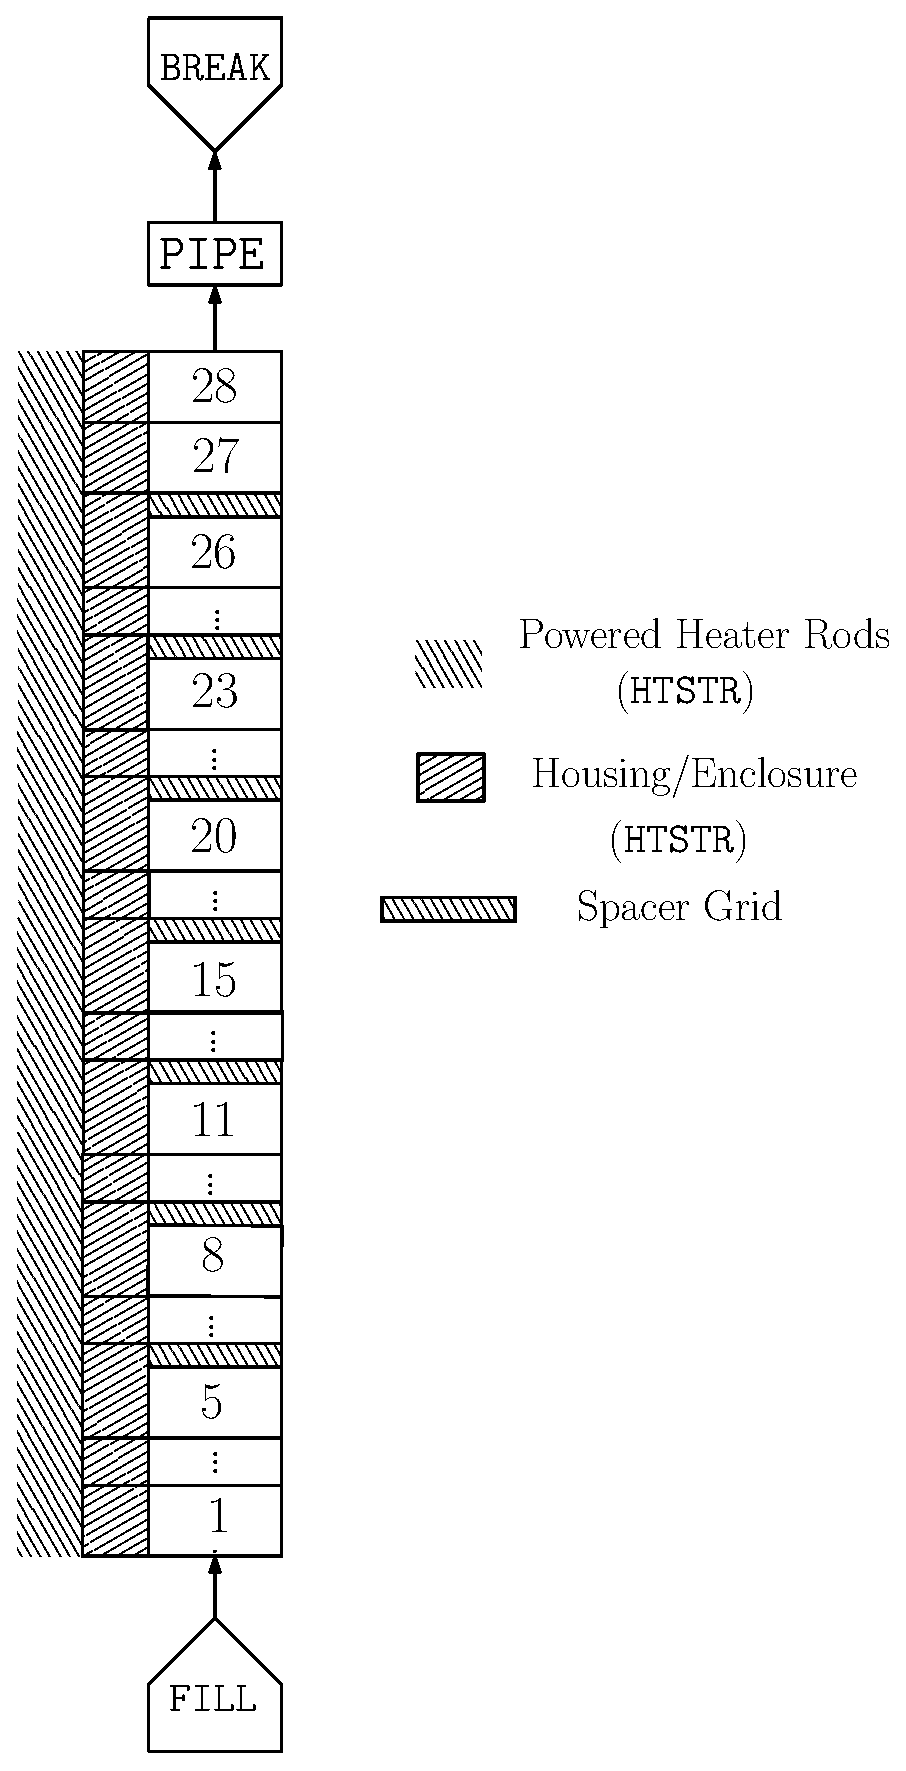
\includegraphics[width=0.65\textwidth]{../figures/chapter2/figures/febaNodalization}
    \caption[Nodalization of the FEBA experimental facility in TRACE.]{Nodalization of the \gls[hyper=false]{feba} experimental facility in \gls[hyper=false]{trace}.}
    \label{fig:ch2_feba_nodalization}
\end{figure}
%******************************************************
\section{Chapter Summary}\label{sec:gp_chapter_summary}
%******************************************************

The functional approximation part of the proposed statistical framework has been presented in this chapter.
The goal of such an approximation was to evaluate the output of a computer simulation code for an arbitrary input much faster.
The approximation is based on Gaussian stochastic process resulting in a statistical metamodel.
As the dimensionality of the output is large, in the order of tens of thousands, a dimension reduction step is adopted by means of \gls[hyper=false]{pca} (an approach similar to what was adopted in Chapter 3).

The results obtained on the \gls[hyper=false]{trace} model \gls[hyper=false]{feba} is reasonable.
Though the prediction error can at times be large, the metamodel gives an overall good performance on average and in context for the three types of multivariate output (clad temperature, pressure drop, and liquid carryover). 
The limitation of the approach is mainly for the output which exhibits strong non-linearity and discontinuity (such as the quenching in the clad temperature transient).
This, in turn, is due to the use of \gls[hyper=false]{pca} as the (linear) dimension reduction tool.
As such, a first step of improvement in this regard can be aimed toward replacing \gls[hyper=false]{pca} with another, more advanced dimension reduction tool.

Using the \gls[hyper=false]{gp} \gls[hyper=false]{pc} metamodel as the surrogate for \gls[hyper=false]{trace} run, 
the prediction for arbitrary model parameters values can be made much faster ($< 5 [s]$ per metamodel evaluation vs. $6-15 \, [min]$ per \gls[hyper=false]{trace} run).
As such the metamodel constructed in this chapter can be used as the basis for Bayesian model calibration which requires tens if not hundreds of thousands function evaluations. 
However, it is also important to note that the time required for the construction of the metamodel and as well as for its convergence study has to be taken into account.
The training, validation, and testing data have to be generated from actual code runs.
Additionally, the model fitting step to estimate \gls[hyper=false]{gp} metamodel hyper-parameters is an optimization problem that can easily become expensive for large training samples of large dimension (large number of input parameters).
 
The study also confirms that the size of the training sample is the main factor in determining the predictive performance of the metamodel.
The choice of covariance function has some impact especially in relation to the stability of the performance,
while the choice of experimental design has a neglible impact on the performance.


\begin{figure}[bth]
    \myfloatalign
    \subfloat[Asia personas duo.]
    {\includegraphics[width=.45\linewidth]{gfx/example_1}} \quad
    \subfloat[Pan ma signo.]
    {\label{fig:example-b}%
        \includegraphics[width=.45\linewidth]{gfx/example_2}} \\
    \subfloat[Methodicamente o uno.]
    {\includegraphics[width=.45\linewidth]{gfx/example_3}} \quad
    \subfloat[Titulo debitas.]
    {\includegraphics[width=.45\linewidth]{gfx/example_4}}
    \caption[Tu duo titulo debitas latente]{Tu duo titulo debitas
        latente. \ac{DRY}}\label{fig:example}
\end{figure}


%*****************************************
%*****************************************
%*****************************************
%*****************************************
%*****************************************
